\documentclass[12pt]{article}
% We can write notes using the percent symbol!
% The first line above is to announce we are beginning a document, an article in this case, and we want the default font size to be 12pt
\usepackage[utf8]{inputenc}
% This is a package to accept utf8 input.  I normally do not use it in my documents, but it was here by default in Overleaf.
\usepackage{amsmath}
\usepackage{amssymb}
\usepackage{amsthm}
% These three packages are from the American Mathematical Society and includes all of the important symbols and operations 
\usepackage{fullpage}
% By default, an article has some vary large margins to fit the smaller page format.  This allows us to use more standard margins.
\usepackage{graphicx}

\setlength{\parskip}{1em}
% This gives us a full line break when we write a new paragraph


\begin{document}
% Once we have all of our packages and setting announced, we need to begin our document.  You will notice that at the end of the writing there is an end document statements.  Many options use this begin and end syntax.

\graphicspath{{figures/}}


\begin{center}
    \Large     Tarea 1 \\ 
    Nahuel Almeira \normalsize
\end{center}

\section{Oscilador arm\'onico}

\subsection{Ecuaci\'on}

En esta pr\'actica resolveremos la ecuaci\'on del oscilador arm\'onico 

\begin{align}\label{eq:oscilador}
\ddot{y} + \omega y &= 0 \nonumber \\
y(0) &= 1 \\
\dot{y}(0) &= 0. \nonumber
\end{align}

Por inspecci\'on, puede verse que la soluci\'on a la ecuaci\'on \ref{eq:oscilador} es 

\begin{equation}
y(t) = \sin(\omega t).
\end{equation}

Para resolver num\'ericamente la ecuaci\'on, conviene transformarla en un sistema de ecuaciones diferenciales de primer orden. Para ello, realizamos el cambio de variables 

\begin{align}
y &= x_1 \\
\dot{y} &= \omega x_2.
\end{align}

As\'i, obtenemos el sistema de ecuaciones 

\begin{equation}
\begin{pmatrix}
\dot{x_1} \\
\dot{x_2}
\end{pmatrix} = 
\begin{pmatrix}
0 & \omega \\
-\omega & 0
\end{pmatrix}
\begin{pmatrix}
x_1 \\
x_2,
\end{pmatrix}
\end{equation}

que podemos escribir como 

\begin{equation}
\dot{x} = A x, \quad x \equiv (x_1, x_2)^T, \quad A \equiv 
\begin{pmatrix}
0 & \omega \\
-\omega & 0
\end{pmatrix}.
\end{equation}

La matriz $A$ es diagonalizable mediante la transformaci\'on

\begin{equation}
A = S^{-1} \Lambda S,\quad S = 
\begin{pmatrix}
i & -i \\
1 & 1
\end{pmatrix},\quad \Lambda = 
\begin{pmatrix}
-i \omega & 0 \\ 
0 & i \omega
\end{pmatrix}.
\end{equation}

Definiendo $\tilde{x} \equiv Sx$, tenemos

\begin{align}
\dot{x} &= A x \nonumber \\
\dot{x} &= S^{-1} \Lambda S x \nonumber\\
S\dot{x} &= \Lambda S x \nonumber \\
\dot{\tilde{x}} &= \Lambda \tilde{x}, \label{eq:diagonal}
\end{align}

con lo cual obtenemos dos ecuaciones desacopladas.

\subsection{M\'etodos num\'ericos}

Para resolver la ecuaci\'on \ref{eq:diagonal} emplearemos dos m\'etodos. El m\'etodo de Euler expl\'icito, de primer orden, y el m\'etodo de Runge-Kutta de orden cuatro (RK4). En ambos casos utilizaremos un paso $k$.

La regi\'on de estabilidad  de cada m\'etodo est\'a relacionada con los autovalres $\lambda$ de $A$. En particular, se debe satisfacer que $|P(\lambda k)|\leq 1$, donde $P$ es un polinomio que depende exclusivamente del m\'etodo. En la figure \ref{fig:estabilidad} se puede comparar la regi\'on de estabilidad para ambos m\'etodos. Los autovalores asociados a la ecuaci\'on a resolver son puramente imaginarios ($\lambda = \pm i \omega$), por lo que es esperable que el m\'etodo de Euler no converja, dado que su regi\'on de estabilidad no incluye el eje imaginario. El m\'etodo RK4, por otro lado, deber\'ia converger para un paso $k$ suficientemente chico.

\begin{figure}
\centering
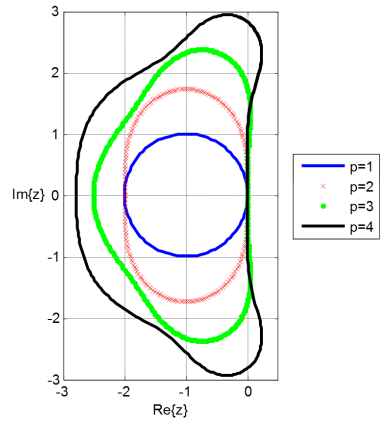
\includegraphics[scale=0.6]{EulerVsRK.png}
\caption{\label{fig:estabilidad} Regi\'on de estabilidad en el plano complejo ($z=\lambda k$) para el m\'etodo de Euler (p=1) y Runge-Kutta (p=4).}
\end{figure}

\subsection{Resultados}

En la figura \ref{fig:oscilador}, se muestra la soluci\'on num\'erica de la ecuaci\'on utilizando los dos m\'etodos. Se puede ver que, mientras que RK4 aproxima muy bien la soluci\'on, Euler es divergente, dando una soluci\'on con una amplificaci\'on a lo largo del tiempo. Se puede ver tambi\'en que la diferencia entre la energ\'ia a tiempo cero y la energ\'ia a tiempo $t$ es considerablemente mayor en Euler que en RK4.

Aunque el m\'etodo de Euler diverge para cualquier valor de $k$, converge a la soluci\'on exacta en el l\'imite $k\rightarrow 0$. Esto se puede ver graficando $|e(T)-e(0)|$ en funci\'on de $k$, para un valor fijo de $T>0$. En la figura \ref{fig:convergencia} se puede ver que la diferencia de energ\'ias disminuye linealmente a medida que se reduce el paso $k$.

\begin{figure}
\centering
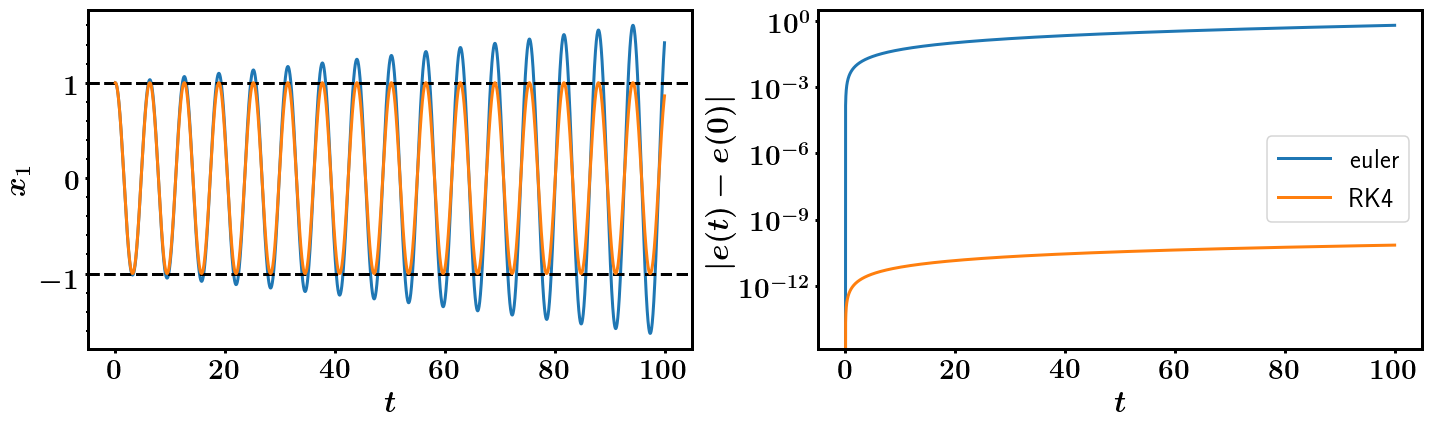
\includegraphics[scale=0.33]{oscilador.png}
\caption{\label{fig:oscilador} Comparaci\'on entre los dos m\'etodos empleados. $k = 0.01$.}
\end{figure}


\begin{figure}
\centering
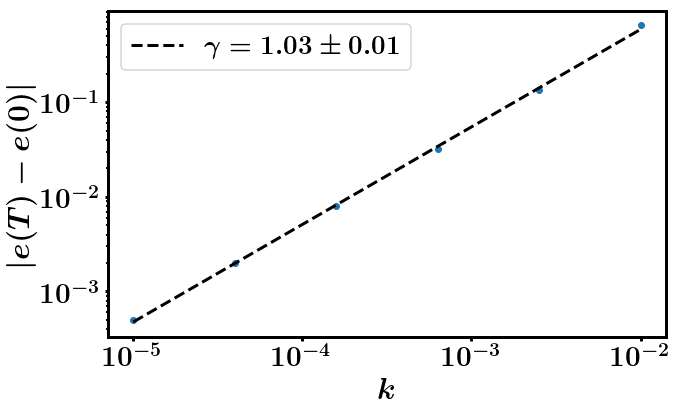
\includegraphics[scale=0.33]{convergencia.png}
\caption{\label{fig:convergencia} Convergencia del m\'etodo de Euler en el l\'imite $k\rightarrow 0$. Se puede ver que $|e(T)-e(0)|\sim k^{\gamma}$, con $\gamma \approx 1$.}
\end{figure}

Para corroborar el orden $p$ de cada m\'etodo, utilizamos la expresi\'on \cite{Kreiss-Ortiz}

\begin{equation}
\tilde{Q} = \dfrac{v_k(t)-v_{k/2}(t)}{v_{k/2}(t)-v_{k/4}(t)} \approx 2^p.
\end{equation}

Podemos ver en la figura \ref{fig:orden} que el orden en cada caso es el correcto

\begin{figure}
\centering
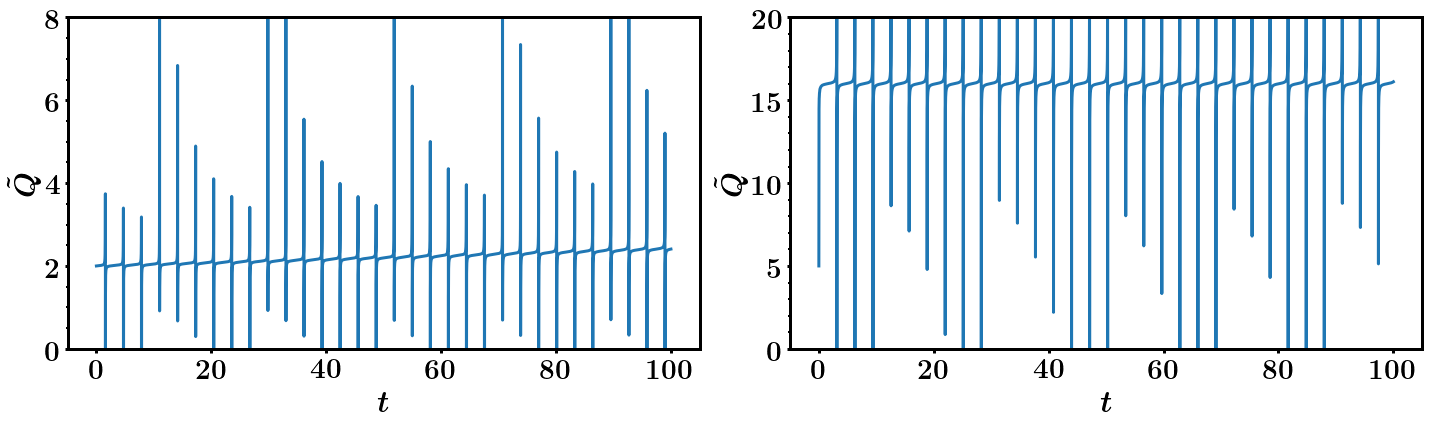
\includegraphics[scale=0.33]{orden.png}
\caption{\label{fig:orden} Corroboraci\'on del orden de cada m\'etodo. Izquierda: Euler; Derecha: RK4.}
\end{figure}

\pagebreak

\section{Potencial central}

\subsection{Ecuaciones}

Resolvemos el problema de una part\'icula de masa unidad sujeta a un potencial central $U(r) = -r^{-1}$. La ecuaci\'on correspondiente es

\begin{equation} \label{eq:central}
\ddot{\mathbf{r}} = -\nabla U(r).
\end{equation}

En coordenadas cartesianas el problema se puede expresar como un sistema de cuatro ecuaciones diferenciales ordinarias 

\begin{equation}
\begin{pmatrix}
\dot{x} \\
\dot{y} \\
\dot{v_x} \\
\dot{v_y}
\end{pmatrix} = 
\begin{pmatrix}
v_x \\
v_y \\
\dfrac{-x}{(x^2 + y^2)^{3/2}} \\
\dfrac{-y}{(x^2 + y^2)^{3/2}}
\end{pmatrix}.
\end{equation}

En cambio, en coordenadas polares, el sistema se reduce a tres dimenciones, ya que una de las ecuaciones resulta trivial. El sistema resulta

\begin{equation}
\begin{pmatrix}
\dot{r} \\
\dot{\phi} \\
\dot{v_r} \\
\dot{v_{\phi}}
\end{pmatrix} = 
\begin{pmatrix}
v_r \\
v_{\phi} \\
-\dfrac{1}{r^2} \\
0
\end{pmatrix}.
\end{equation}

La energ\'ia mec\'anica del sistema est\'a dada por 

\begin{equation}
E = T + U = \dfrac{1}{2} \bigg( \dot{r}^2 + r^2 \dot{\phi}^2 \bigg) - \dfrac{1}{r}.
\end{equation}

La energ\'ia, que es una cantidad conservada del sistema, determina el tipo de \'orbita que tiene lugar. Para $E<0$, las \'orbitas son elipses (acotadas), mientras que para $E>0$, las \'orbitas son hip\'erbolas (no acotadas). El caso $E=0$ da lugar a \'orbitas parab\'olicas.

Utilizamos las condiciones iniciales 

\begin{align}
x(0) &= 1 \\
y(0) &= 0 \\
v_x(0) &= 0 \\
v_y(0) &= v,
\end{align}

con $v > 0$. Con estas condiciones, la energ\'ia mec\'anica es $E = v^2/2 - 1$. Luego, la condici\'on para tener \'orbitas cerradas es $v < \sqrt{2}$.

En la figura \ref{fig:cartesianas}, se muestra la resoluci\'on num\'erica del sistema (en coordenadas cartesianas) para distintas energ\'ias, utilizando el m\'etodo RK4 con $k = 0.01$. Vemos que la energ\'ia se mantiene acotada siempre y cuando la velocidad inicial no sea demasiado baja. 

\begin{figure}
\centering
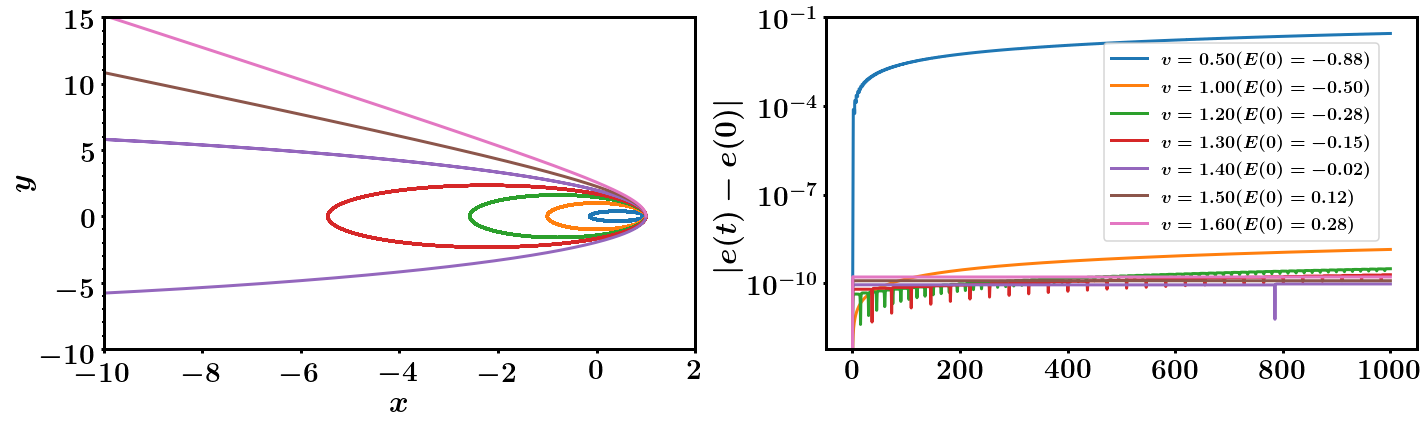
\includegraphics[scale=0.3]{cartesianas.png}
\caption{\label{fig:cartesianas} Soluciones al sistema \ref{eq:central}, con coordenadas cartesianas, para diferentes energ\'ias. $k = 0.01$.}
\end{figure}

%Cuando la energ\'ia es negativa, pero cercana a cero, las soluciones num\'ericas presentan una inestabilidad. Tal como se puede ver en la figura \ref{fig:precesion}, en lugar de una \'orbita cerrada, lo que se ve es una \'orbita que presenta una precesi\'on.

Por \'ultimo, analizamos el comportamiento asint\'otico de las soluciones (utilizando coordenadas polares). En la figura \ref{fig:last_phi} se muestra el valor de $\phi(T=1000)$ para distintas condiciones iniciales de $v_r$, correspondientes a \'orbitas abiertas con energ\'ias cercanas a cero. Se puede ver que, independientemente de la condici\'on inicial, las \'orbitas alcanzan el mismo valor angular.

\begin{figure}
\centering
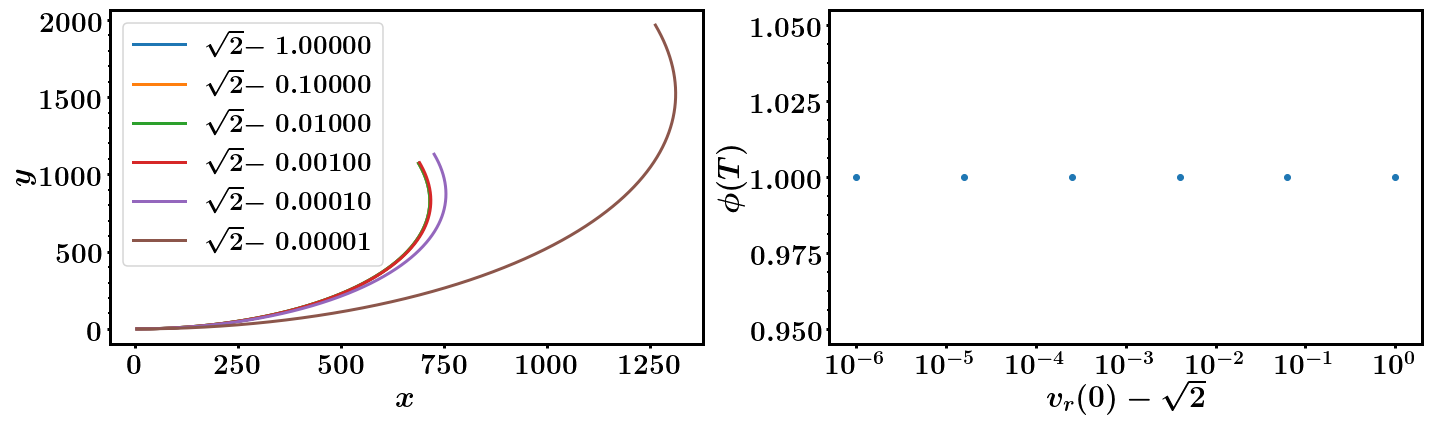
\includegraphics[scale=0.3]{last_phi.png}
\caption{\label{fig:last_phi} \'Orbitas abiertas con $E\approx 0$. Se observa que, para el mismo tiempo $T=1000$, todas las soluciones terminanan en el mismo \'angulo.}
\end{figure}


%%%%%%%%%%%%%%%%%%%%%%%%%%%%%%%%%%%%%%%%%%%%%%%%%

\begin{thebibliography}{1}

\bibitem{Kreiss-Ortiz} {\em Introduction to Numerical Methods for Time Dependent Differential Equations}, H. Kreiss and O. Ortiz, (2014).

\end{thebibliography}


\end{document}
